\chapter{Présentation des fonctionnalités}
Lorsque l'on lance notre Pong, un menu s'affiche. Celui-ci présente 2 modes que l'on explicitera par la
suite, le mode « Solo » et le mode « Multijoueur ». Le premier se présentant comme une extension au but 
du projet initial et possédant des règles spécifiques, nous allons d'abord nous concentrer sur le mode multijoueur.


\section{Multijoueur}

Le mode multijoueur est celui qui exploitera le réseau. Les 2 joueurs doivent lancer le Pong et l'un d'entre eux 
doit sélectionner « Serveur » dans le menu déroulant, après avoir choisi le mode multijoueur et la valeur du score à atteindre 
pour gagner la partie. La partie ``nom du serveur'' ne le concerne pas. Ainsi, son 
application se met en attente d'un client, soit le deuxième joueur. Ce dernier doit sélectionner « Client » 
et doit indiquer le nom de la machine sur laquelle il souhaite se connecter, soit son IP. La partie ``score max''
ne le concerne pas. Le jeu se 
lance alors en même temps pour les 2 joueurs.
\\
Par défaut, le joueur de gauche est celui qui a sélectionné le serveur, et le client est le joueur de 
droite. Une balle apparaît au centre du jeu et se dirige arbitrairement sur lui. Par la suite, après chaque point 
marqué, le jeu se stoppe 1 seconde afin de marquer une pause entre chaque point et d'actualiser clairement 
le score, puis une nouvelle balle apparaît dans la direction du joueur ayant encaissé un point.
\\
Cependant, le jeu ne s'arrête pas là. Un ensemble de « balles bonus » a été mis en place. Celles-ci 
ont des couleurs et une forme différentes, les distinguant de la balle de jeu originale. Elles apparaissent 
selon un rythme régulier, selon le score. En effet, le score des 2 joueurs est régulièrement additionné, et 
tous les x points (x correspondant à la valeur indiquée dans la colonne « Rythme » ci-dessous), la balle 
bonus correspondante apparaît au centre de l'écran et se dirige vers la dernière personne ayant marqué un 
point s'il s'agit d'un bonus, son adversaire s'il s'agit d'un malus. 
Leurs effets respectifs disparaîssent après 2 tours.

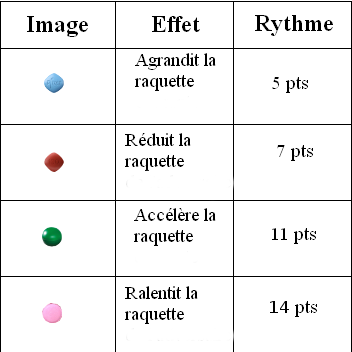
\includegraphics[scale=0.5]{./images/pilules.png}


\subsection{Le réseau}

Le premier joueur est serveur lorsque l'on lance le jeu, cependant la communication se fait dans 
les 2 sens entre les joueurs, serveur et client. Tout d'abord, lorsque le premier joueur lance le jeu, il 
envoie la valeur de son score max au possible client qui se connecterait. Lorsque celui-ci arrive, il 
reçoit le score max et renvoie une chaîne de caractères servant d'accusé de réception (noté ``ack'' dans 
la suite du rapport).
Ensuite, à chaque instant, chacun des joueurs envoie 
la position courante de sa raquette à l'adversaire qui peut ainsi positionner la raquette de son 
adversaire de son point de vue, afin d'être sûr que les 2 applications soient synchronisées. La balle 
est également synchronisée, cependant, pour pouvoir régulièrement vérifier si les valeurs envoyées 
sont les bonnes, les 2 joueurs gèrent la balle à tour de rôle. Lorsque la balle se situe sur la 
première moitié gauche de l'écran, le joueur 1 doit calculer la position et la vitesse de la balle et les envoyer 
au joueur 2 qui peut ainsi récupérer les valeurs et déplacer la balle sur son application à la 
position correspondante, ainsi que lui attribuer la bonne vitesse. Si la balle est sur la moitié droite de l'écran,
c'est ainsi le joueur 
2 qui gère la balle et le joueur 1 qui reçoit les informations, de façon similaire. Les raquettes et la balle 
ont également un système d'ack qui garantit l'envoi des données.
\\
Les données sont envoyées selon un format particulier et suivent le protocole suivant. Une fonction ``send'' 
envoie les données, l'autre joueur les reçoit dans une fonction ``read'' et renvoie un ack qui sera réceptionné 
dans une fonction ``ack''. Si la fonction ``ack'' retourne ``true'', l'envoi et la réception se sont effectués 
correctement, sinon, on renvoie les données. Chacun des trois objets à synchroniser (les raquettes, la balle et 
le score max) le sont à l'aide des fonctions send/read différentes qui seront explicitées plus tard. La fonction ``ack'' 
quant à elle est générique et s'adapte à tous les objets. Voici le format des données qui sont envoyées:

\begin{itemize}
 \item \textit{Coordonnées de la racket: ``x\_racket''double ou ``y\_racket''double}
 \item \textit{Position de la balle: ``x\_ballpos``double ou ''y\_ballpos``double}
 \item \textit{Vitesse de la balle: ''x\_ballspeed``double ou ''y\_ballspeed``double}
 \item \textit{Score max: ''score``int}
\end{itemize}

Ainsi, le nom de l'objet envoyé est un String, et est suivi de la donnée elle-même. La fonction read appelée correspondante 
effectue d'abord la fonction ''readObject`` afin de récupérer le String et vérifie si la valeur récupérée correspond à 
celle attendue. Si tel est le cas, la fonction ''read`` spécifique au type d'objet suivant est appelée et la variable 
à synchroniser est modifiée. Par la suite, la fonction read envoie le message servant d'ack qui est, selon le type de donnée 
envoyé, l'un des suivants:

\begin{itemize}
 \item \textit{Coordonnées de la racket: ``x\_racket\_recu'' ou ``y\_racket\_recu''}
 \item \textit{Ball position: ``x\_ballpos\_recu`` ou ''y\_ballpos\_recu``}
 \item \textit{Ball speed: ''x\_ballspeed\_recu`` ou ''y\_ballspeed\_recu``}
 \item \textit{Score max: ''score\_recu``}
\end{itemize}

L'envoi de chacune des données est contenue dans une boucle ''do while`` de la sorte:

\begin{lstlisting}[language=Java]
do{
	r.send(sock, ballData[0], "x_ballpos");
}while(!r.ack(sock, "x_ballpos_recu"));
do{
	r.send(sock, ballData[0], "y_ballpos");
}while(!r.ack(sock, "y_ballpos_recu"));
do{
	r.send(sock, ballData[1], "x_ballspeed");
}while(!r.ack(sock, "x_ballspeed_recu"));
do{
	r.send(sock, ballData[1], "x_ballspeed");
}while(!r.ack(sock, "x_ballspeed_recu"));
\end{lstlisting}

Ainsi, l'envoi s'est effectué correctement si la chaîne de caractère souhaitée en ack, celle passée en paramètre, 
a été envoyée, la fonction ''ack`` retournant donc ''true``. Sinon, 
on renvoie les données.

\section{Solo}

Nous avons jugé intéressant de ne pas seulement faire un mode multijoueur mais également d'intégrer un mode solo, 
qui donc ne fait forcément pas appel au réseau, auquel nous avons intégré des règles spécifiques.
\\
Pour le lancer, il suffit de sélectionner ''Solo`` dans ''Mode de jeu`` et de lancer la partie à l'aide de ''Play``. 
Les options suivantes ne servent qu'en mode ''Multijoueur``. Le joueur se retrouve face à une raquette, contrôlée par l'IA, 
imbattable. Il est en effet impossible pour lui de marquer un point comme dans le mode multijoueur, car la raquette 
en face calcule la coordonnée y de la balle et se positionne selon elle, lui permettant ainsi de la réceptionner en permanence. 
Le score du joueur est ainsi calculé par le nombre de fois où il arrive à renvoyer la balle. Son score est augmenté de 1 
à chaque rebond et repart à 0 lorsque celui-ci se prend un point. Ce mode solo peut ainsi être vu comme un mode entraînement.

\section{Jeux de tests}

Nos tests sont situés dans la classe Tests.java et on peut les effectuer en lançant le programme avec pour argument 
la chaîne de caractères 
''test``.
Ici, le menu ne se lancera pas mais les tests seront fait automatiquement et l'utilisateur verra s'afficher sur la sortie 
standard le message suivant: ''"Les tests ont été passés avec succès``, si les tests se passent sans problèmes.
Nous avons décidé de créer des tests sur des fonctions jugées fondamentales et complexes, afin d'être sûr que celles-ci 
agissent de la façon attendue, et ce quels que soient les cas. Nous avons ainsi choisi les fonctions ''collision`` et 
''rebound``, situées toutes deux dans la classe ''Pong.java``.
\\
La méthode est similaire pour les 2. Nous lançons un parcours composé de 4 boucles ''for``, la première sélectionnant 
la première puis la deuxième raquette, la deuxième modifiant la trajectoire y de la raquette courante et les 2 suivantes 
bougeant la balle dans l'espace en x et y. Ainsi, nous testons toutes les positions possibles de la balle en fonction de 
toutes les positions possibles de chaque raquette, indépendamment l'une de l'autre. Dans chaque cas, nous vérifions 
si la fonction à tester retourne bien les paramètres attendus. Nous comparons ainsi les résultats dits ''expérimentaux``, 
correspondant aux valeurs réelles, celles obtenues de par les objets ''Pong`` et ''Ball`` créés, avec les résultats 
attendus, c'est-à-dire les valeurs souhaitées dans les fonctions tests.

